\documentclass {report}
\usepackage{float}
\usepackage{longtable}
\usepackage{color}
\usepackage{appendix}
\usepackage{hyperref}
\hypersetup{
    colorlinks=true, % make the links colored
    linkcolor=black, % color TOC links in black
    urlcolor=red, % color URLs in red
    linktoc=all % 'all' will create links for everything in the TOC
}
\usepackage{graphicx}
\graphicspath{{images/}}
\usepackage{csquotes}
\usepackage{fancyvrb}

\usepackage[backend=bibtex,style=numeric]{biblatex}
%\bibliography{sources} 
\addbibresource{sources.bib}

\title {
	{sidBison: A Stepwise Interactive Debugger for Bison\\[0.4in]}
	{ Tufts University\\[0.2in]}
	{\large Advisor: Prof. Kathleen Fisher\\}
}

\author {Siddhartha Prasad}
\date{23rd March 2016}

\begin {document}

\maketitle

\thispagestyle{plain}
\begin{center}
    \textbf{Abstract}
\end{center}

Parser-generator systems specifications are generally large and hard to debug. Generated code often does not semantically match the programmers intent. Debugging machine-generated parsers is a non-trivial task, requiring knowledge of underlying implementations. This has led to the decline of bottom-up parser-generators as staples in language design and syntactic analysis workbenches.\\

Stepwise Interactive Debugger for Bison is a step-through debugger that preserves an abstraction boundary between Bison specifications and the underlying parser tables. It allows a user to debug a Bison 2.3 specification at the grammar level, requiring minimal knowledge of bottom-up parsing. The ultimate goal of this project is to make parser-generating tools more accessible to the average programmer.

\pagebreak
\tableofcontents
\pagebreak

\thispagestyle{plain}
\begin{center}
    \textbf{A Quick Note}
\end{center}

\noindent

This thesis is aimed at audiences who have previously encountered formal grammars and/or concrete syntax trees.
Appendix A contains a quick introduction to formal and context-free grammars.\\

Familiarity with parser-generators like \verb|Yacc| or \verb|Bison| is not required, but will allow for deeper understanding of the problem. I recommend reading the Bison user manual at \verb|http://www.gnu.org/software/bison/manual/|.

\pagebreak

\chapter{Introduction}

\section{Machine generated parsers}

A parser is a machine that examines a string of characters and acts in response to those characters according to the rules of a formal grammar. In computing, parsers have widespread applications, ranging from Natural Language Processing to compiler generation. Programmers often use these systems to translate information into formats about which they can reason more easily.\\

Early parsers were common well before a theory of formal grammars was developed, and were painstakingly written into punchcards. With Backus and Naur's formalization of \emph{Extended Backus Naur Form} (EBNF) notation for describing languages, programs were soon contracted for this tedious job. Recursive-descent parser generating machines soon became the standard, allowing programmers to put in grammars and get out entire parsers \cite{Bidwell}. While these top-down methods were easily understandable and debuggable, the generated machines could not deal with several everyday scenarios, including left-recursion. This led to the generation of \textbf{Bottom Up} parsing methods and their generators. These systems could process most common grammars, and preserved the EBNF abstraction afforded earlier to programmers. However, in doing so, these programs became very complex, involving several tables, automata and stacks. Programmers soon could not easily explain the underlying mechanisms of these systems.

Modern parser-generators produce lots of hard-to-understand code. If the resulting parser does not semantically match the programmer's intent, debugging the system is a non-trivial task. Examining errors in specifications requires knowledge of the underlying code-generating implementation. This thesis introduces a tool that attempts to make the parser-generation process more accessible to the average programmer by offering the ability to step-through and debug grammar specifications.


\section{Bison}

Bison is a very popular bottom-up (LALR) parser generator that was built for the GNU project as an alternative to Yacc. According to the GNU website:

\begin{displayquote}
Bison is a general-purpose parser generator that converts an annotated context-free grammar into a deterministic LR or generalized LR (GLR) parser employing LALR(1) parser tables. As an experimental feature, Bison can also generate IELR(1) or canonical LR(1) parser tables. Once you are proficient with Bison, you can use it to develop a wide range of language parsers, from those used in simple desk calculators to complex programming languages.\textit{- GNU Bison} \citation{GNU}
\end{displayquote}

\subsection{Basic Actions}

The \verb|Bison| parser-generator employs a \textit{bottom-up} parsing mechanism \cite{UnderstandingBison}. The program uses an input specification to generate a push-down automaton as well as a token stack. It executes transitions between states on based on the tokens encountered. \verb|Bison| has three basic actions \cite{Appel} \cite{BisonAlgorithm}:

\begin{enumerate}

\item \textbf{shift}: As Bison encounters input tokens, it pushes them onto the token stack.
\item \textbf{reduce}: When the last $k$ shifted tokens match a rule, they are merged to form the non-terminal specified in the left hand side of the rule. This symbol is now stored on the token stack. The push-down automata then pops back to a previous state.
\item \textbf{lookahead}: \verb|Bison| often \emph{looks ahead} at the next coming token before performing a shift or reduce action, in order to better ascertain what to do.
\end{enumerate}

\verb|Bison| attempts to use shifts and reductions (with the aid of lookaheads) to match input to a specified \textit{start} symbol in the specification \cite{BisonAlgorithm}.

\subsection{Lookaheads}
While the need for a lookahead may not be apparent, the following example shows its effectiveness.

\begin{Verbatim}[frame=single]
	Digit : 1 | 2 | 3

	Number : Digit 
                 | Digit Number
\end{Verbatim}

On input \verb|12| the parser requires the look-ahead to know that after the digit $1$ has been shifted, it should not immediately be reduced to the rule \verb|Number|.


\subsection{Limitations}

While Bison is able to produce parsers for a wide range of grammars, its underlying LALR(1) parser table implementation
is limited to certain forms. Certain specifications can cause shift-reduce and reduce-reduce conflicts, where there is ambiguity in
what action should be executed \cite{LRWiki}.

\subsubsection{Shift-Reduce Conflicts}

\begin{Verbatim} [frame=single]
    E -> a E
          | a
\end{Verbatim}

In the grammar above, we see that when parsing terminal \verb|a|, there could be a reduce action to \verb|E|
and a shift action in order to parse the rule \verb|a E|. In such a situation, an LR parser would not be able to decide on a \lq correct\rq option. \verb|BISON| shifts in such a situation, which may not echo the programmers intent \cite{BisonAlgorithm}.

\subsubsection{Reduce-Reduce conflicts}


\begin{Verbatim} [frame=single]
    X -> Y a | Z b
    Y -> a
    Z -> a
\end{Verbatim}

In the grammar above, we see that the terminal \verb|a| could be reduced to \verb|Y| or \verb|Z|. Bottom-up parsers like \verb|BISON| do not have a resolution strategy in such a situation \cite{DonnellyandStallman}.


\section{Programmer Errors}

Real-world Bison specifications are often very large. Much like any other language, larger specifications create greater room for programmer error. As a result, while generated parsers may accept input, they often do not behave in a way intended by programmers. Debugging these machine-generated parsers is a non-trivial task. While Bison provides error messaging in terms of the underlying parser implementation, it is not easy to examine the semantics of a specification. A user needs to be familiar not only with the specified grammar, but also LR parsing to correct errors in their code.

The following are \verb|Bison| specifications that do not accept the exact set of strings a programmer might expect.

\subsection{Small Specifications: Calculator Language}

This section looks at a grammar specification for a simple calculator language \cite{DonnellyandStallman} that accepts integers and performs addition, subtraction, multiplication and division. While this grammar may seem to specify the calculator language at first, it cannot parse any string with more than one operator. For instance, the string \verb|1 + 1 + 1| is not accepted.

\begin{Verbatim} [frame=single]

	Digit : 1 
            | 2
            | 3
            | 4
            | 5
            | 6
            | 7
            | 8
            | 9
            | 0

	Number : Digit 
                 | Digit Number
	
	Operator : + 
                  | -
                  | *
                  | /
	
	Expression : Number
                   | Number Operator Number

\end{Verbatim}

\subsection{Large Specifications: JSON}

Larger grammars, by virtue of their size, are hard to debug. The specification in \textbf{Appendix 6.3} is intended to describe JSON strings \cite{BrayTim}. Upon closer inspection, one might notice that the grammar can parse only 2 members with value separators. 
Identifying which rule causes the error requires traversing almost the the whole grammar. A step-though debugging approach can be hard to execute manually.\\

As a result of the complexity of these systems, parser generators like Bison are quickly losing ground to other parsing approaches. An influential paper by Matthew Might and David Darais claims that Yacc is dead \cite{Yaccisdead}. Increasing the accessibility of these systems could help bottom up parser generators re-emerge as a staple of the average language designer's workbench.  


\chapter{Stepwise Interactive Debugger for Bison}


\verb|iBison| is a version of \verb|Bison 2.3| that was built by S.K. Popuri at the University of Illinois at Chicago. It generates 
an interactive interface that allows a user to step through the parsing process, presenting information in terms of a push-down automaton and its state and token stacks \cite{iBison}. Stepwise Interactive Debugger for Bison (sidBison), leverages this responsive design to allow for debugging at the grammar level. The system is modelled on \verb|gdb|-style debuggers, allowing for not only the identification of errors in \verb|Bison| specifications but also those in input strings, maintaining an abstraction barrier between grammars and parser-generated state tables.\\

The goal of this project is to simplify the parser-generation process for programmers who are not well-versed with the underlying implementation. Debuggers preserving such abstraction barriers could be particularly useful in the process of democratizing language design workbenches.

\section{Using sidBison}

The \verb|sidBison| system requires a \verb|Bison| specification and lexer shared object in order to debug a string. A more detailed setup process as well as examples are described in Appendix B.

\section{Commands}

The \verb|sidBison| command set is designed to reinforce the abstraction barrier between a Bison specification and the underlying parser implementation.

\begin{enumerate}
\item \textbf{crule}: Returns the current non-terminal rule being parsed in the Bison specification.
\item \textbf{steprule} : Steps to the next rule in the Bison specification
\item \textbf{str}: Identifies the current position in the entire parsing process.
\item \textbf{br} : Allows the user to break when a particular token is encountered.
\item \textbf{step} : Steps to the next action taken by the parser
\item \textbf{ctkn} : Displays the current token being looked at by the parser.
\item \textbf{rulepos} : Identifies current position in the rule being parsed.
\item \textbf{test $<$filename$>$} : Accepts the input string as a file.
\item \textbf{quit} : Ends the sidBison program
\end{enumerate}

The implementation of these commands is described in the Chapter 3: \textit{Implementing sidBison Commands}.

\section{Usability}

\verb|sidBison|'s success hinges on its usability. It should be able to aid a user with the examples presented earlier. This is predicated on the idea that:

\begin{enumerate}
\item Humans generally find EBNF easier to understand than push-down automata.
\item The ability to step through grammar specifications presents bottom-up parsing in an understandable, linear manner.
\end{enumerate}

These criteria are evaluated in the case study presented in Chapter 5: \textit{Case Study: Usability}.





\chapter{Implementing sidBison Commands}

\verb|sidBison| is designed to be a step-through debugger at the grammar level, and is built on top of \verb|iBison|'s interactive debugging mechanism. The mathematical underpinnings of the system involve mapping \verb|Bison| and \verb|iBison| constructs like 
\begin{enumerate}
\item Push-Down Automata
\item State Stacks
\item Token Stacks
\item Lookaheads
\end{enumerate}
\noindent
to Extended Backaus Naur Form (EBNF) grammar rules. As a result, each command takes the form of a mathematical function in terms of these variables. Thus, \verb|sidBison| commands can be thought of as a set $\{ f_i \}$ of functions.

\paragraph{step}

The \verb|step| command allows the user to step forward to the next action taken by the underlying parser debugger. It is the simplest command for the \verb|sidBison| system. The rule is of the form $f_1(ss, ts, ct) \rightarrow (ss', ts', tc')$, where:

\begin{enumerate}
\item $ss$ and $ss'$ are state stacks, where $ss'$ is a new state stack created by taking a step.
\item $ts$ and $ts'$ are token stacks, where $ts$ is a new token stack created by taking a step.
\item $ct$  and $ct'$ are current tokens, where $ct'$ is a new current token obtained either by a new lookahead or from $ss'$.
\end{enumerate}

\verb|step| provides the basis of mapping actions in terms of the underlying parser to those involving \verb|Bison| specifications. It maps a new \textit{lookahead} to encountering a new token, a shift to adding the token to the string, and a reduce to parsing a string. Several of the more complicated \verb|sidBison| commands leverage \verb|step|.

\paragraph{steprule}

The \verb|steprule| command takes the user to the next rule encountered by the parser. Thus, it presents a step-wise debugging abstraction in terms of the user-provided grammar specification instead of parser-generator options. 

The command is implemented by stepping through \verb|iBison| state changes till a reduce action is executed. As a result
it has the mathematical form $f_2: \verb|Parser Automaton| \rightarrow (ss`, ts`)$, where :

\begin{enumerate}
\item $ss'$ represents a new state stack, and by extension a new current state.
\item $ts'$ represents a new token stack.
\end{enumerate}

\paragraph{crule}

The \verb|crule| command returns the current rule being parsed by Bison generated parser. It takes the form of a mathematical function \\ $f_3: (\mbox{Parser Automaton},  $cs$  , $ss$) \rightarrow (\mbox{Backus Naur Form Rule})$, where $cs$ is the current state, and $ss$ is the state stack.\\

In general, a bottom-up parser cannot predict the non-terminal to which a partially known sequence of tokens will be reduced. Even judging if a reduction will ever take place is an undecidable problem. As a result, the command cannot be implemented using a single instance of a single-pass parser like \verb|Bison|. \verb|crule| therefore utilizes a time-travelling heuristic.

This approach is concurrent in nature. A secondary \verb|iBison| process is spawned and is placed in the same state as the primary one. This secondary debugger is then stepped forward to the first parser \textit{reduce} action where the state stack has either shrunk, or has the same size with a different top element. The reduced rule is precisely the production being parsed.

\paragraph{rulepos}

\verb|rulepos| enumerates current positions the parser may be in within grammar rules. It is implemented by examining the rules
and positions associated with the current rule in the underlying automaton. It has the mathematical form $f_4: cs \rightarrow [(\mbox{Backus Naur Form Rule},  p)]$, where $cs$ represents the current state and $p$ represents a position in the rule.

\paragraph{str}

The \verb|str| command returns the current position in the overall parsing process. It is implemented by displaying the contents of the \verb|iBison| token stack. It has mathematical form $f_5: cs \rightarrow str_{ss}$, where $cs$ represents the current state and $str_{ss}$ is a string representation of the state stack.

\paragraph{ctkn}

The \verb|ctkn| command displays the token with which the parser is currently dealing. It is implemented by presenting the newer of the look-ahead token and the top element of the token stack.


\paragraph{br}

The \verb|br| command allows the user to break when a particular token is encountered. This functionality is provided by stepping till the \verb|ctkn| equals the token provided. Thus it has mathematical form $f_6 : tkn \rightarrow (cs', ss')$, where:

\begin{enumerate}
\item $ss'$ represents a new state stack, and by extension a new current state.
\item $ts'$ represents a new token stack.
\item $tkn$ represents the input token.
\end{enumerate}


The \textbf{quit} and \textbf{test} commands are not involved in the actual debugging process, and so are not explained above.


\chapter{Interactivity}

The \verb|sidBison| tool cannot be considered a successful stepwise debugger if it is not truly interactive. As a result, each command must execute in a resonable amount of time. Since a command's execution time may be context dependent, an understanding of the system's time-complexity may help users improve their use of the system. These analytical formulae, along with empirical run-times,
also allow for the evaluation of the interactivity of \verb|sidBison|.

\section{Complexity}

\paragraph{Complexity of Bison}

It is necessary to understand the runtime of Bison before reasoning about \verb|sidBison|'s runtime. According to the Bison user manual, "a GLR parser can take quadratic or cubic worst-case time, and the current Bison parser even takes exponential time and space for some grammars" \cite{LinearBison}. However, for most grammars parsing time is $O(|G| n)$ \cite{LinearBison}\cite{ComplexityGLR}. $|G|$ is the number of tokens in the grammar and $n$ is the length of the string to be parsed.

\paragraph{Reading from iBison}

\verb|sidBison| is built on top of Satya Kiran Popuri's \verb|iBison| system. As a result, much of \verb|sidBison|'s resources and run-time are invested in inter-process communication. Several commands read information from the iBison process. As a result, it is important to compute the asymptotic time needed to communicate with iBison.

\begin{enumerate}
\item  The size of information output from \verb|iBison| is a function of its state and token stack sizes.
\item \verb|sidBison| sets an upper limit of $1 KB$ on the sizes of the state and token stacks.
\item As a result, there is a fixed upper bound on the information that needs to be read from iBison.
\end{enumerate}

Thus, while the constants in question may be large (at most $2 KB$), reading information from iBison takes $O(1)$ time.
This communication is implemented in the  function \verb|read_from_ibison|.

\paragraph{step}

The \verb|step| command is the most basic of \verb|iBison| commands. It executes a single Bison step. Since reading from iBison takes constant time, \verb|step|'s run-time has complexity $O(n|G|)$ where $n = 1$. Since the number of tokens in a grammar is constant for any debugging instance, step runs in constant time. 

\paragraph{steprule}

The \verb|steprule| command steps repeatedly till a reduce action is executed. Thus, it may call \verb|step| up to $n$ times, where $n$ is the length of the input string. As a result, since the number of tokens in a grammar is constant for any debugging instance, it has complexity $O(n)$.

\paragraph{ctkn}

The \verb|ctkn| command accesses the newer of the top element of the token stack and the lookahead to return the current token. As both these operations take constant time, \verb|ctkn| runs in $O(1)$.

\paragraph{str}

The \verb|str| command returns the contents of the token stack. As the size of this stack is bounded, it runs in $O(1)$.

\paragraph{br}

The \verb|br| command steps repeatedly till the current token equals a specified token. Thus, it may call \verb|step|  and \verb|ctkn| up to $n$ times each, where $n$ is the length of the input string. As both \verb|step| and \verb|ctkn| take constant time, it has complexity $O(n)$.

\paragraph{crule}

The time-travelling \verb|crule| command spawns a new \verb|iBison| process and steps first to the current state, and then till the current rule is reduced. As a result, it steps and reads from iBison  up to $n$ times, where $n$ is the length of the input string. As a result, it runs in $O (n)$. However, given that it has to spawn a new process, the constants in the linear describing its execution time are large.

\paragraph{rulepos}

The \verb|rulepos| command helps identify the user's current position in the rule they are parsing. It first looks up the rules associated with the current parser automaton state and then calls \verb|crule|. As looking up rules is a constant time operation, and \verb|crule| is linear, the \verb|rulepos| command runs in $O(n)$.\\



\section{Empirical analysis}

Compiling \verb|sidBison| with the \verb|DDEBUGLOG=1| flag enables a timing routine with least count $10^{-6}$ seconds . This feature writes system and user time taken by a command to \verb|stderr|. Runtimes for each command were logged while debugging examples in Appendix C. Raw data can be found in Appendix D.



\begin{figure}[H] \centering
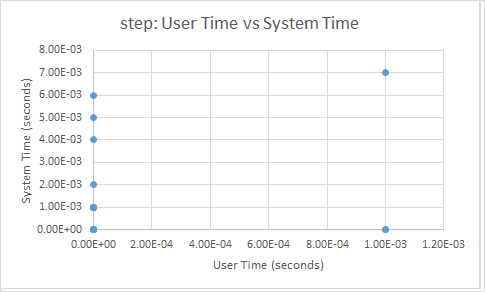
\includegraphics[height=6cm,width=10cm]{step.png}
\end{figure}

\noindent

The average user time taken by the \textbf{step} command was $1.07*10^{-4}s$ with standard deviation $3.150 * 10^{-4} s$. The average system  time taken was $1.29*10^{-3} s$ with standard deviation $1.883 * 10^{-3} s$\\.


\begin{figure}[H] \centering
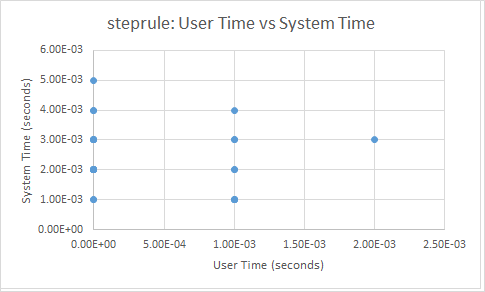
\includegraphics[height=6cm,width=10cm]{steprule.png}
\label{fig:steprule}
\end{figure}

\noindent

The average user time taken by the \textbf{steprule} command was $3.33*10^{-4} s$ with standard deviation $ 5.34*10^{-4}s$. The average system time taken was $2.31 * 10^{-3} s$ with standard deviation $9.80* 10^{-4} s$\\.


\begin{figure}[H] \centering
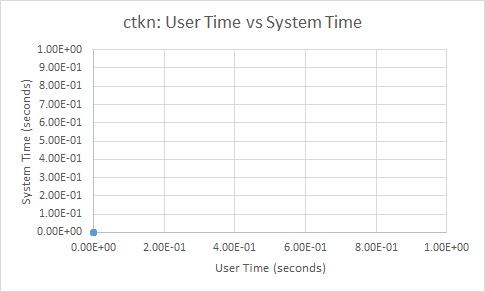
\includegraphics[height=6cm,width=10cm]{ctkn.png}
\end{figure}

\noindent

The average user time taken by the \textbf{ctkn} command was $0 s$ with standard deviation $0 s$. The average system  time taken was $0 s$ with standard deviation $0 s$\\.


\begin{figure}[H] \centering
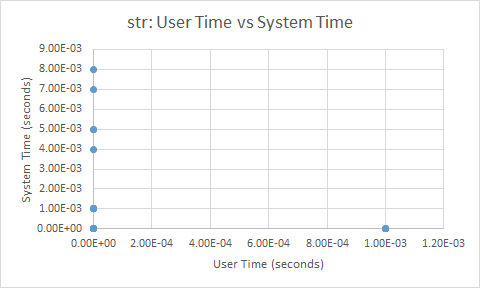
\includegraphics[height=6cm,width=10cm]{str.png}
\end{figure}

\noindent

The average user time taken by the \textbf{str} command was $1.18 * 10^{-4} s$ with standard deviation $3.270 * 10^{-4} s$. The average system  time taken was $1.12 * 10^{-3} s$ with standard deviation $2.1 * 10^{-3} s$\\.


\begin{figure}[H] \centering
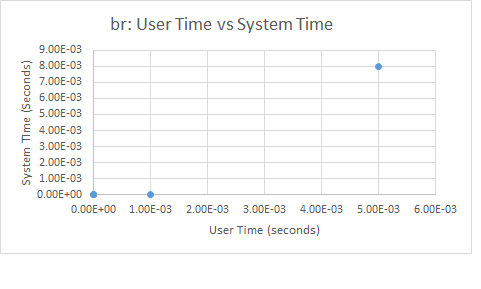
\includegraphics[height=6cm,width=10cm]{br.png}
\end{figure}

\noindent

The average user time taken by the \textbf{br} command was $1.20 * 10^{-3} s$ with standard deviation $2.168 * 10^{-3} s$. The average system time taken was $1.60 * 10^{-3} s$ with standard deviation $3.577 * 10^{-3} s$\\.


\begin{figure}[H] \centering
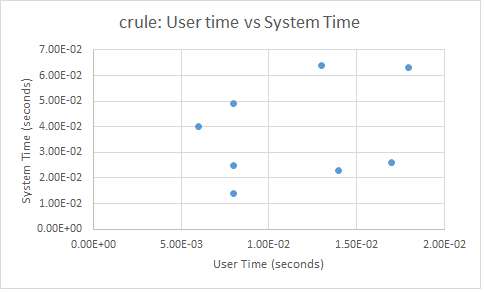
\includegraphics[height=6cm,width=10cm]{crule.png}
\end{figure}

\noindent

The average user time taken by the \textbf{crule} command was $1.15 * 10^{-2} s$ with standard deviation $4.597 * 10^{-3} s$. The average system  time taken was $3.80 * 10^{-2} s$ with standard deviation $1.9046 * 10^{-2} s$\\.

\begin{figure}[H] \centering
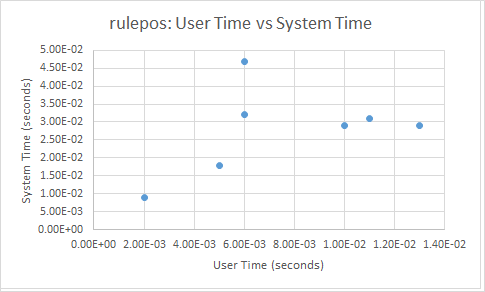
\includegraphics[height=6cm,width=10cm]{rulepos.png}
\end{figure}

\noindent

The average user time taken by the \textbf{rulepos} command was $7.57 * 10^{-3} s$ with standard deviation $3.866 * 10^{-3} s$. The average system time taken was $2.79 * 10^{-2} s$ with standard deviation $1.18930 ^ 10^{-3} s$\\.

\section{Conclusion}

All \verb|sidBison| commands run in either constant or linear time in the average case. While constants might be large, this guarantees that the system's response time will not grow too large as input string sizes increase. Maximum average execution times for grammar are of the order $10^{-3} s$  for $O(1)$ commands and $10^{-2} s$ for $O(n)$ commands, with low standard deviations. If grammar sizes increase, \verb|sidBison|'s command execution time will only grow linearly -- the same as GNU Bison. Thus, debugging tool promises to deliver reasonable execution times for reasonably sized grammars. 



\chapter{Case Study : Usability}

\textbf{Note: This is a study proposal}\\

The ultimate goal of the \verb|sidBison| project is to make parser-generating tools more accessible to the average programmer. The proposed study will study the effectiveness of Stepwise Interactive Debugger for Bison as a tool that aids this accessibility. This will be achieved by studying its helpfulness in performing tasks with the Bison parser-generator. While ease of use and intuitiveness are very hard to quantify, user case studies are a good way to get a sense for the system's effectiveness.

The proposed  study will involve student volunteers from the Computer Science department at Tufts University. In addition to graduate students, undergraduate upperclassmen, especially those who are in or have taken Comp 181: Compilers and Comp 105: Programming Languages will also be approached to participate in the study via the online class forums. The only identifying information that will be collected will be the subject's level of familiarity with parser-generator systems.

Subjects will be provided with incorrect parser-generator specifications and inputs, and will be asked to debug these programs with and without \verb|sidBison|.  A questionnaire will then be administered, evaluating the intuitiveness and ease of use of the tool. 

The anonymous, statistical results of the survey will be included in the final thesis.




\chapter{Using sidBison}

This section presents a small example of using \verb|sidBison|. Given a \verb|Flex| file \verb|lexer.l|, and a \verb|Bison| file \verb|parser.y|, a lexer shared object  \verb|lex.so| can be prepared for input to \verb|sidBison| as follows:

\begin{Verbatim} [frame=single]

ibison -d parser.y
flex lexer.l   
gcc -c -fPIC lex.yy.c
gcc -shared -o lex.so lex.yy.o

\end{Verbatim}

This requires the \verb|LD_LIBRARY_PATH| environment variable to include the directory in which \verb|lexer.so| is available and the \verb|BISON_PKGDATADIR| variable points to the \verb|ibison\data| directory. \verb|sidBison| can now be run with \verb|parser.y| and \verb|lex.so| as command-line arguments.

\section{Lambda Calculus}

The lambda calculus example described in Appendix B involves files \href{https://github.com/sidprasad/sidbison/blob/master/lambdacalcexample/lambdacalc.l}{lambdacalc.l} and \href{https://github.com/sidprasad/sidbison/blob/master/lambdacalcexample/lambdacalc.y}{lambdacalc.y}.

\paragraph{Compilation} These files can be compiled to create a lexer shared object file for input for \verb|sidBison| as described below..

\begin{Verbatim} [frame=single]

ibison -d lambdacalc.y
flex lambdacalc.l   
gcc -c -fPIC lex.yy.c
gcc -shared -o lex.so lex.yy.o

\end{Verbatim}

After compilation, the generated files can be loaded into \verb|sidBison| as command line arguments.

\begin{Verbatim} [frame=single]

./sidbison lambdacalc.y lex.so

\end{Verbatim}

\subsection{Debugging input}

The file \href{https://github.com/sidprasad/sidbison/blob/master/lambdacalcexample/input/ycombinator.err} {ycombinator.err} contains the string \verb|\h.(\h.(\x.(h (x x))) \x.(h (x x)))|. This is not accepted by the specified lambda calculus grammar. An example step-through debug is described below.\\


\textbf{Want screenshots and step through process}

\section{Impcore}

\section{Source Code}

Source code for \verb|sidBison| be found at \url{https://github.com/sidprasad/sidbison/}. 

\noindent
Example Flex and Bison specifications can be found in Appendix B.

\noindent
 Source code and instructions for building and installing iBison can be found at \url{https://www.cs.uic.edu/~spopuri/ibison.html}.

\chapter{Additional Work}

The ultimate aim of this project is to make parser-generator systems more accessible. 
\begin{enumerate}
\item The \verb|sidBison| system could be expanded to deal with LL parser generator systems such as ANTLR. 
\item \verb|sidBison| could also be ported to \verb|YACC| implementations in languages such as C++, F \# and Standard ML.
\item Syntax highlighting and IDE support for Bison files could help improve the readability and debug-ability of grammar specifications.
\item Just-In-Time compiling within an IDE could help highlight potential conflicts in the specification while it is being written.

\end{enumerate}

\begin{appendices}


\chapter{A Quick Overview of Formal Grammars}

A formal grammar is a set of rules that describe how strings might be produced in a language.  It can function as both a recognizer and a language generating construct. 

\paragraph{Terminals}

Terminal symbols are actual members of the alphabet that compose the language described by a formal grammar.

\paragraph{Non-terminals}

Non-terminal symbols can be thought of as textit{syntactic variables} that describe groupings or combinations of other symbols, as described by the rules of a formal grammar.

\section{Context Free Grammars}

A context-free grammar is a special kind of formal grammar where each rule is of the form $E \rightarrow \alpha$, where $E$ is a non-terminal symbol and $\alpha$ is a string of terminals and non-terminals in the grammar. Such a grammar is not context dependent -- the non-terminal symbol $E$ can always be replaced by $\alpha$, regardless of the situation.\\

\textbf{Backus Naur Form} (BNF) is a notational method used to describe context-free grammars. It has the basic form
$E := \alpha \mid \beta \ldots$ \cite{BNF}. Here, the non-terminal $E$ could be replaced either by the strings $\alpha$ or $\beta$. Thus, the BNF specification for a language $\{a\}^{*}$ is

\begin{Verbatim}[frame=single]

E  :=  E a
       | a

\end{Verbatim}

\verb|Bison| specifications are rooted in Backus Naur Form.





\chapter{Examples}

\section{Calculator}
\label{appendix:calculator}
Presented below are Flex and Bison files that represent a calculator.  These specifications were inspired by an \verb|iBison| example \cite{iBison}. These files can be debugged with \verb|sidBison| are presented below.

\subsection{Lexer file: calcparser.l}

\begin{Verbatim}[frame=single]

%{                                            
# include "calcparser.tab.h"
# undef yywrap
# define yywrap() 1
%}

%option noyywrap

int   [0-9]+
blank [ \t]

%%
{blank}+
[\n]+      
\+	   return OPERATOR_PLUS;
-	   return OPERATOR_MINUS;
\*	   return OPERATOR_MULT;
\/	   return OPERATOR_DIV;
\(	   return LPAREN;
\)	   return RPAREN;
{int}      return NUMBER;
.          {fprintf(stderr,"Invalid token!\n");}
%%

\end{Verbatim}

\subsection{Grammar file: calcparser.y}

\begin{Verbatim}[frame=single]

%{
/* A simple calculator */
void yyerror(const char *s);
%}
%token        NUMBER
%token 	      OPERATOR_PLUS
%token	      OPERATOR_MINUS
%token	      OPERATOR_MULT
%token 	      OPERATOR_DIV
%token	      LPAREN
%token 	      RPAREN
%left OPERATOR_PLUS OPERATOR_MINUS
%left OPERATOR_MULT OPERATOR_DIV
%%
exp: exp OPERATOR_PLUS exp
   | exp OPERATOR_MINUS exp
   | exp OPERATOR_MULT exp 
   | exp OPERATOR_DIV exp
   | LPAREN exp RPAREN
   | NUMBER
;
%%
void
yyerror(cosnt char *s)
{
  fprintf(stderr,"Syntax error: %s\n",s);
}

\end{Verbatim}


\section{Programmable Computable Functions}

PCF is a simple typed functional language proposed by Dana Scott in 1969.  Flex and Bison files that can be debugged with \verb|sidBison| are presented below.

\subsection{Lexer file: pcf.l}

\begin{Verbatim}[frame=single]
%{
# include "pcf.tab.h"
# undef yywrap
# define yywrap() 1

%}

%option noyywrap

blank [ \t]
word [a-zA-Z][a-zA-Z0-9]*


%%
{blank}+
[\n]+
0           return ZERO;
:           return COLON;
"true"      return TRUE;
"false"     return FALSE;
\.          return DOT;
\(          return LPAREN;
\)          return RPAREN;
"fix"       return FIX;
"zero"      return ZEROFUNC;
"succ"      return SUCC;
"pred"      return PRED;
"if"        return IF;
"then"      return THEN;
"else"      return ELSE;
"fn"        return FN;
"nat"       return NAT;
"bool"      return BOOL;
"->"        return ARROW;
{word}      return IDEN;
.           {fprintf(stderr, "Invalid token!\n");}

%%
\end{Verbatim}

\subsection{Parser file: pcf.y}

\begin{Verbatim}[frame=single]
%{

/* A simple PCF grammar */

%}

%token ZERO
%token TRUE
%token FALSE
%token IDEN
%token FIX
%token ZEROFUNC
%token LPAREN
%token RPAREN
%token SUCC
%token PRED
%token IF
%token THEN
%token ELSE
%token FN
%token COLON
%token DOT
%token NAT
%token ARROW
%token BOOL

%left ARROW

%%


m : ZERO
  | TRUE
  | FALSE
  | var
  | zerofunc
  | succ
  | pred
  | ifelse
  | fun
  | app
  | fix

fix : FIX LPAREN m RPAREN

app : LPAREN callfunc argfunc RPAREN

callfunc : m
argfunc : m


tau : NAT
    | BOOL
    | funtau
    | LPAREN funtau  RPAREN

funtau : tau ARROW tau


fun : FN var COLON tau DOT m

succ : SUCC LPAREN m RPAREN

pred : PRED LPAREN m RPAREN

zerofunc : ZEROFUNC LPAREN m RPAREN

var : IDEN

ifelse : IF m THEN m ELSE m

%%
/*

app : funcexp argexp

succ : SUCC LPAREN m RPAREN
pred : PRED LPAREN m RPAREN
fix : FIX LPAREN m RPAREN

funcexp : m
argexp : m

fix : LPAREN m RPAREN

func : FN var COLON tau DOT m

*/
void yyerror (const char *s)
{
fprintf(stderr, "Syntax error: %s\n", s);
}
\end{Verbatim}

\section{Lambda Calculus}
\label{appendix:lambdacalc}
The lambda calculus is a formal system that expresses computation by way of functions. Flex and Bison files that can be debugged with \verb|sidBison| are presented below.

\subsection{Lexer file: lambdacalc.l}

\begin{Verbatim}[frame=single]
%{
# include "lambdacalc.tab.h"
# undef yywrap
# define yywrap() 1

%}

%option noyywrap

blank [ \t]
word [a-zA-Z][a-zA-Z0-9]*
int [0-9]+


%%
{blank}+
[\n]+
{int}       return CONSTANT;
{word}      return IDENT;
\.          return DOT;
\\          return LAMBDA;
\(          return LPAREN;
\)          return RPAREN;
.           {fprintf(stderr, "Invalid token!\n");}

%%
\end{Verbatim}

\subsection{Grammar file: lambdacalc.y}

\begin{Verbatim}[frame=single]

%{
/* Untyped lambda calculus */
void yyerror(const char *s);

%}

%token  IDENT
%token  CONSTANT
%token  LPAREN
%token  RPAREN
%token  LAMBDA
%token  DOT

%%

exp : var
    | func
    | app
    | CONSTANT

func : LAMBDA var DOT scope

app : LPAREN funcexp argexp  RPAREN

scope : exp

funcexp : exp

argexp : exp

var : IDENT


;

%%
void
yyerror(const char *s)
{
    fprintf(stderr, "Syntax error: %s\n", s);
}

\end{Verbatim}

\section{Impcore}

Impcore is a simple imperative language used as a pedagogical tool in Comp 105: Programming Languages at Tufts University. A lexer and parser for impcore are presented below:

\subsection{Lexer file: imp.l}

\begin{Verbatim}[frame=single]
%{
#include "heading.h"
# include "imp.tab.h"
# undef yywrap
# define yywrap() 1

/* Need to include - in word */

%}

%option noyywrap

blank [ \t]
word [a-zA-Z][a-zA-Z0-9\-]*
int [0-9]+


%%
{blank}+
[\n]+
\(              return LPAREN;
\)              return RPAREN;
\+              return PLUS;
-               return MINUS;
\*              return MUL;
\/              return DIV;
"="             return EQ;
\<              return LT;
\>              return GT;
"val"           return VAL;
"define"        return DEFINE;
"use"           return USE;
"check-expect"  return CHECKEXPECT;
"set"           return SET;
"if"            return IF;
"while"         return WHILE;
"begin"         return BEGN;
"print"         return PRINT;
"check-err"     return CHECKERR;
{int}           {return NUMERAL;}
{word}          {return NAME;}
.               {fprintf(stderr, "Invalid token!\n");}

%%

\end{Verbatim}

\subsection{Parser file: imp.y}
\begin{Verbatim}[frame=single]
%{
/* Leaving unit-test out of def */
#include "heading.h"
#include <stdio.h>
void yyerror(const char *s);
int yylex(void);
%}


%token  VAL
%token  DEFINE
%token  LPAREN
%token  RPAREN
%token  USE
%token  CHECKEXPECT
%token  SET
%token  IF
%token  WHILE
%token  BEGN
%token  PLUS
%token  MINUS
%token  MUL
%token  DIV
%token  EQ
%token  LT
%token  GT
%token  PRINT
%token  CHECKERR
%token  NUMERAL
%token  NAME




%%


program : 
        | def program

def : LPAREN VAL variablename exp RPAREN                                         | exp     
    | LPAREN DEFINE functionname formals exp RPAREN
    | LPAREN USE filename RPAREN                     
    | unittest  


unittest : LPAREN CHECKEXPECT exp exp RPAREN     
          | LPAREN CHECKERR exp RPAREN    

exp : literal                             
    | variablename                        
    | LPAREN SET variablename exp RPAREN  
    | LPAREN IF exp exp exp RPAREN          
    | LPAREN WHILE exp exp RPAREN         
    | LPAREN BEGN expstar                           
    | LPAREN function expstar                       



expstar : RPAREN                                    
        | exp expstar                                
                                                     

formals : LPAREN variablenamestar                  

variablenamestar : RPAREN                           
                  | variablename variablenamestar 


literal : NUMERAL           

function : functionname           
         | primitive              

primitive : PLUS                  
          | MINUS                                 
          | MUL                    
          | DIV                    
          | EQ                     
          | LT                     
          | GT                     
          | PRINT                  

variablename : NAME 
functionname : NAME 
filename : NAME  


;

%%
void
yyerror(const char *s)
{
    fprintf(stderr, "Syntax error: %s\n", s);
}

\end{Verbatim}

\section{JSON Grammar}

\begin{Verbatim} [frame=single]
    JSON-text : ws value ws

	begin-array     : ws %x5B ws  ; [ left square bracket

	begin-object    : ws %x7B ws  ; { left curly bracket

	end-array       : ws %x5D ws  ; ] right square bracket

	end-object      : ws %x7D ws  ; } right curly bracket

	name-separator : ws %x3A ws  ; : colon

	value-separator : ws %x2C ws  ; , comma


	ws  :	               ; Empty string
		   | %x20 |            ; Space
		   %x09 |              ; Horizontal tab
		   %x0A |              ; Line feed or New line
		   %x0D                ; Carriage return

	value : false | null | true | object
			 | array | number | string

	false : %x66.61.6c.73.65   ; false

	null  : %x6e.75.6c.6c      ; null

	true  : %x74.72.75.65      ; true

	object : begin-object
	      [ member ( value-separator member ) ]
			end-object

	member : string name-separator value

	array : begin-array [ value *( value-separator value ) ]
				 end-array

	number : [ minus ] int [ frac ] [ exp ]

	decimal-point : %x2E       ; .

	digit1-9 : %x31-39         ; 1-9

	e : %x65 | %x45            ; e E

	exp : e [ minus | plus ] 1*DIGIT

	frac : decimal-point 1*DIGIT

	int : zero | ( digit1-9 *DIGIT )

	minus : %x2D               ; -

	plus : %x2B                ; +

	zero : %x30                ; 0

	string : quotation-mark *char quotation-mark

	char : unescaped 
		   | escape (
		   %x22 |          ; "    quotation mark  U+0022
		   %x5C |          ; \    reverse solidus U+005C
		   %x2F |          ; |    solidus         U+002F
		   %x62 |          ; b    backspace       U+0008
		   %x66 |          ; f    form feed       U+000C
		   %x6E |          ; n    line feed       U+000A
		   %x72 |          ; r    carriage return U+000D
		   %x74 |          ; t    tab             U+0009
		   %x75 4HEXDIG )  ; uXXXX                U+XXXX

	escape : %x5C              ; \

	quotation-mark : %x22      ; "

	unescaped : %x20-21 | %x23-5B | %x5D-10FFFF
\end{Verbatim}


\chapter{Empirical Data}

\begin{center}
\begin{longtable}{|l|l|l|}
\caption[Raw DDEBUGLOG Data]{Raw DDEBUGLOG Data} \label{grid_mlmmh} \\

\hline \multicolumn{1}{|c|}{\textbf{Command}} & \multicolumn{1}{c|}{\textbf{User Time (s)}} & \multicolumn{1}{c|}{\textbf{System Time (s)}} \\ \hline 
\endfirsthead

\multicolumn{3}{c}%
{{\bfseries \tablename\ \thetable{} -- continued from previous page}} \\
\hline \multicolumn{1}{|c|}{\textbf{Command}} &
\multicolumn{1}{c|}{\textbf{User Time (s)}} &
\multicolumn{1}{c|}{\textbf{System Time (s)}} \\ \hline 
\endhead

\hline \multicolumn{3}{|r|}{{Continued on next page}} \\ \hline
\endfoot

\hline \hline
\endlastfoot

br                            & 5.00E-03      & 8.00E-03        \\
br                            & 0.00E+00      & 0.00E+00        \\
br                            & 0.00E+00      & 0.00E+00        \\
br                            & 0.00E+00      & 0.00E+00        \\
br                            & 9.99E-04      & 0.00E+00        \\
crule                         & 8.00E-03      & 2.50E-02        \\
crule                         & 1.40E-02      & 2.30E-02        \\
crule                         & 6.00E-03      & 4.00E-02        \\
crule                         & 8.00E-03      & 4.90E-02        \\
crule                         & 8.00E-03      & 1.40E-02        \\
crule                         & 1.70E-02      & 2.60E-02        \\
crule                         & 1.30E-02      & 6.40E-02        \\
crule                         & 1.80E-02      & 6.30E-02        \\
ctkn                          & 0.00E+00      & 0.00E+00        \\
ctkn                          & 0.00E+00      & 0.00E+00        \\
ctkn                          & 0.00E+00      & 0.00E+00        \\
ctkn                          & 0.00E+00      & 0.00E+00        \\
ctkn                          & 0.00E+00      & 0.00E+00        \\
ctkn                          & 0.00E+00      & 0.00E+00        \\
ctkn                          & 0.00E+00      & 0.00E+00        \\
ctkn                          & 0.00E+00      & 0.00E+00        \\
ctkn                          & 0.00E+00      & 0.00E+00        \\
ctkn                          & 0.00E+00      & 0.00E+00        \\
ctkn                          & 0.00E+00      & 0.00E+00        \\
rulepos                       & 6.00E-03      & 3.20E-02        \\
rulepos                       & 2.00E-03      & 9.00E-03        \\
rulepos                       & 1.00E-02      & 2.90E-02        \\
rulepos                       & 1.30E-02      & 2.90E-02        \\
rulepos                       & 6.00E-03      & 4.70E-02        \\
rulepos                       & 5.00E-03      & 1.80E-02        \\
rulepos                       & 1.10E-02      & 3.10E-02        \\
step                          & 0.00E+00      & 0.00E+00        \\
step                          & 0.00E+00      & 0.00E+00        \\
step                          & 0.00E+00      & 1.00E-03        \\
step                          & 0.00E+00      & 0.00E+00        \\
step                          & 0.00E+00      & 1.00E-03        \\
step                          & 0.00E+00      & 5.00E-03        \\
step                          & 0.00E+00      & 0.00E+00        \\
step                          & 1.00E-03      & 0.00E+00        \\
step                          & 0.00E+00      & 1.00E-03        \\
step                          & 0.00E+00      & 6.00E-03        \\
step                          & 0.00E+00      & 0.00E+00        \\
step                          & 0.00E+00      & 1.00E-03        \\
step                          & 9.99E-04      & 7.00E-03        \\
step                          & 0.00E+00      & 0.00E+00        \\
step                          & 0.00E+00      & 4.00E-03        \\
step                          & 0.00E+00      & 1.00E-03        \\
step                          & 0.00E+00      & 9.99E-04        \\
step                          & 0.00E+00      & 1.00E-03        \\
step                          & 0.00E+00      & 1.00E-03        \\
step                          & 0.00E+00      & 1.00E-03        \\
step                          & 0.00E+00      & 0.00E+00        \\
step                          & 0.00E+00      & 2.00E-03        \\
step                          & 0.00E+00      & 1.00E-03        \\
step                          & 0.00E+00      & 1.00E-03        \\
step                          & 0.00E+00      & 1.00E-03        \\
step                          & 1.00E-03      & 0.00E+00        \\
step                          & 0.00E+00      & 0.00E+00        \\
step                          & 0.00E+00      & 0.00E+00        \\
steprule                      & 1.00E-03      & 2.00E-03        \\
steprule                      & 0.00E+00      & 3.00E-03        \\
steprule                      & 0.00E+00      & 3.00E-03        \\
steprule                      & 0.00E+00      & 1.00E-03        \\
steprule                      & 1.00E-03      & 4.00E-03        \\
steprule                      & 0.00E+00      & 3.00E-03        \\
steprule                      & 1.00E-03      & 3.00E-03        \\
steprule                      & 0.00E+00      & 2.00E-03        \\
steprule                      & 9.99E-04      & 1.00E-03        \\
steprule                      & 0.00E+00      & 2.00E-03        \\
steprule                      & 0.00E+00      & 2.00E-03        \\
steprule                      & 1.00E-03      & 1.00E-03        \\
steprule                      & 0.00E+00      & 2.00E-03        \\
steprule                      & 0.00E+00      & 2.00E-03        \\
steprule                      & 1.00E-03      & 2.00E-03        \\
steprule                      & 1.00E-03      & 9.99E-04        \\
steprule                      & 0.00E+00      & 4.00E-03        \\
steprule                      & 1.00E-03      & 3.00E-03        \\
steprule                      & 0.00E+00      & 4.00E-03        \\
steprule                      & 0.00E+00      & 3.00E-03        \\
steprule                      & 1.00E-03      & 1.00E-03        \\
steprule                      & 0.00E+00      & 2.00E-03        \\
steprule                      & 0.00E+00      & 3.00E-03        \\
steprule                      & 0.00E+00      & 2.00E-03        \\
steprule                      & 0.00E+00      & 2.00E-03        \\
steprule                      & 1.00E-03      & 1.00E-03        \\
steprule                      & 0.00E+00      & 2.00E-03        \\
steprule                      & 0.00E+00      & 1.00E-03        \\
steprule                      & 0.00E+00      & 2.00E-03        \\
steprule                      & 0.00E+00      & 2.00E-03        \\
steprule                      & 0.00E+00      & 2.00E-03        \\
steprule                      & 0.00E+00      & 2.00E-03        \\
steprule                      & 0.00E+00      & 5.00E-03        \\
steprule                      & 2.00E-03      & 3.00E-03        \\
steprule                      & 0.00E+00      & 2.00E-03        \\
steprule                      & 0.00E+00      & 3.00E-03        \\
stprule                       & 0.00E+00      & 0.00E+00        \\
str                           & 0.00E+00      & 0.00E+00        \\
str                           & 0.00E+00      & 9.99E-04        \\
str                           & 0.00E+00      & 1.00E-03        \\
str                           & 1.00E-03      & 0.00E+00        \\
str                           & 0.00E+00      & 0.00E+00        \\
str                           & 0.00E+00      & 9.99E-04        \\
str                           & 1.00E-03      & 0.00E+00        \\
str                           & 0.00E+00      & 1.00E-03        \\
str                           & 0.00E+00      & 0.00E+00        \\
str                           & 1.00E-03      & 0.00E+00        \\
str                           & 0.00E+00      & 0.00E+00        \\
str                           & 0.00E+00      & 1.00E-03        \\
str                           & 0.00E+00      & 5.00E-03        \\
str                           & 0.00E+00      & 0.00E+00        \\
str                           & 0.00E+00      & 0.00E+00        \\
str                           & 1.00E-03      & 0.00E+00        \\
str                           & 0.00E+00      & 1.00E-03        \\
str                           & 0.00E+00      & 7.00E-03        \\
str                           & 0.00E+00      & 0.00E+00        \\
str                           & 0.00E+00      & 0.00E+00        \\
str                           & 0.00E+00      & 9.99E-04        \\
str                           & 0.00E+00      & 0.00E+00        \\
str                           & 0.00E+00      & 4.00E-03        \\
str                           & 0.00E+00      & 0.00E+00        \\
str                           & 0.00E+00      & 1.00E-03        \\
str                           & 0.00E+00      & 0.00E+00        \\
str                           & 0.00E+00      & 0.00E+00        \\
str                           & 0.00E+00      & 5.00E-03        \\
str                           & 0.00E+00      & 0.00E+00        \\
str                           & 0.00E+00      & 0.00E+00        \\
str                           & 0.00E+00      & 1.00E-03        \\
str                           & 0.00E+00      & 0.00E+00        \\
str                           & 0.00E+00      & 8.00E-03        \\
str                           & 0.00E+00      & 0.00E+00  		\\  
\end{longtable}
\end{center}

\end{appendices}

\printbibliography

\end{document}



